\documentclass{article}
\usepackage{listings}
\usepackage[utf8]{inputenc}
\usepackage{ amssymb }
\usepackage{amsfonts}
\usepackage{graphicx}


\title{Sistemas Distribuidos y Verificación \\ Tarea 9}
\author{Fabián Romero Jiménez}
\date{}
\begin{document}

\maketitle

\begin{enumerate}

\item[\bf{Problema 1}] Los programadores de la compañía de computación Flaky diseñaron el
protocolo que se muestra a continuación para lograr la exclusión mútua de n-hilos. 
Para cada pregunta, presenta una prueba o despliega una ejecucción donde falle.

(Aquí invertí las lineas 11 y 12 de la tarea enviada, puesto que no era sintacticamente correcto).

\lstset{numbers=left, stepnumber=1, numbersep=5pt}
\begin{lstlisting}
class Flaky implements Lock {
  private volatile int turn;
  private volatile boolean busy = false;
  public void lock(){
    int me = ThreadID.get();
    do{
      do{ 
        turn = me ;
      } while(busy);
      busy = true;
    } while (turn != me);
  }
  public void unlock(){
    busy = false;
  }
}
\end{lstlisting}


\begin{itemize}
\item ¿El protocolo satisface la exclusión mútua?\\

Sí.
\item Demostración\\
Supongamos que no, entonces hay un momento en el tiempo $T_{both}$ en donde ambos están en su sección crítica, por lo que ambos leyeron $busy=false$, por lo que ambos escribieron $turn=me$ digamos que en  $T_{me1}$ y $T_{me2}$ respectivamente, observe que en cualquier momento $turn!=me$ sólo puede ser cierto para uno de los procesos, pero debe de ser cierto para ambos en $T_{both}$ que es posterior a  $T_{me1}$ y $T_{me2}$ lo cual contradice nuestra hipótesis.

\item ¿Este protocolo es starvation-free?\\
No
\item Demostración\\
 probaremeos en el siguiente apartado que no es deadlock-free, y por lo tanto cualquier ejecución que caiga en deadlock provoca starvation.

\item ¿Este protocolo es deadlok-free?\\
No
\item Demostración\\
Demos un ejemplo de ejecución que causa deadlock.\\
Empieza la ejecución con el recurso libre, entonces entran dos procesos $A$ y $B$ y digamos que $A$ corre hasta la linea 9 y ahí se atonta un poco, en ese momento llega $B$ hasta la linea 8, por lo que se tendrá que $turn=B$, en eso $A$ despierta y ejecuta la linea 10 $busy=true$ y al llegar a la linea 11 se queda atorado en el while pues el turno no es de el, en tanto $B$ llega a la línea 9 y se atorado en el while pues $busy=true$ y así entran en deadlock.

\end{itemize}


\item[\bf{Problema 2}]Durante la exposición se mostró la construcción de un sistema bounded-timestamp para 2 y 3 hilos, con base en la explicación dada, construya uno para 4 hilos y responda adicionalmente las siguientes preguntas.

\begin{center}
  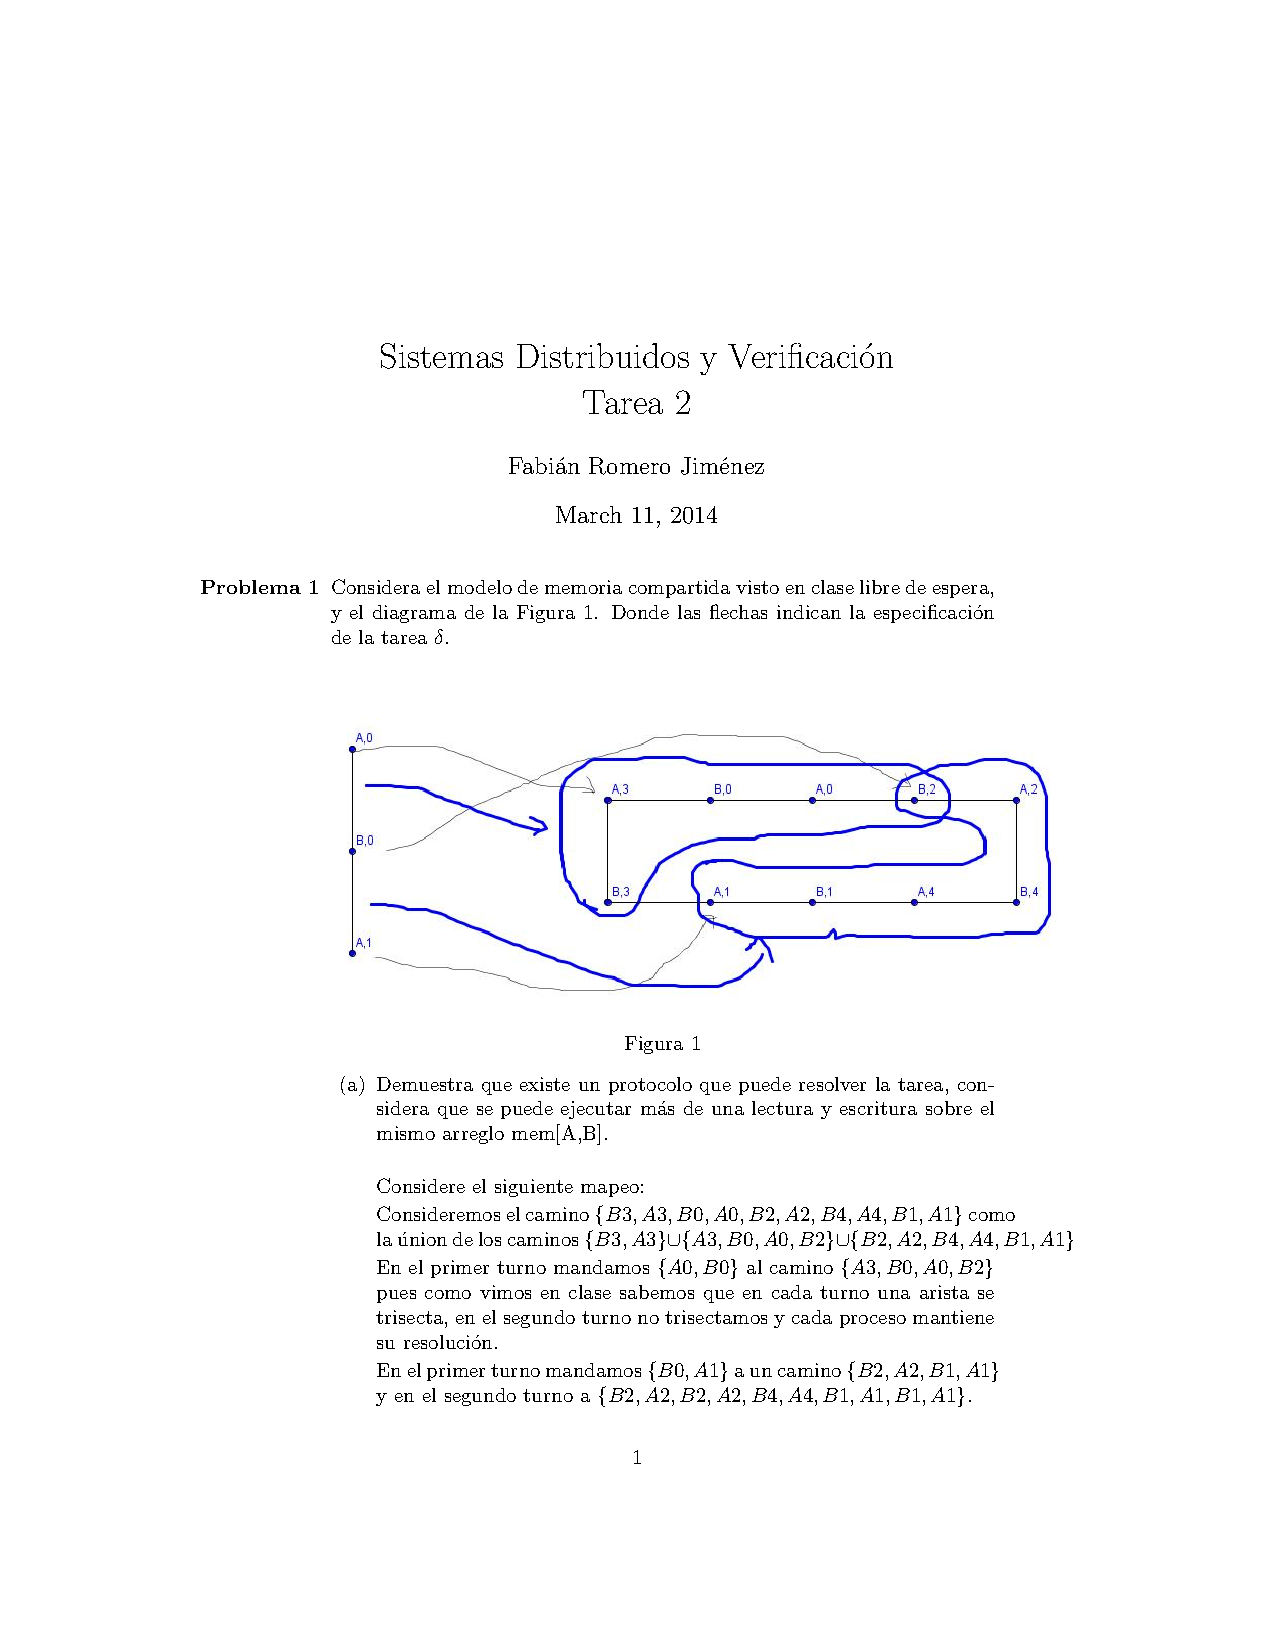
\includegraphics[width=350pt]{t4.png}\\
  T4
\end{center}

\begin{itemize}
\item En el sistema construido para 3 hilos puede observarse que existen
más vértices que procesos y podría suponerse que es posible
el utilizarlo para 4 hilos, muestre un ejemplo que contradiga esta
suposición.
\begin{center}
  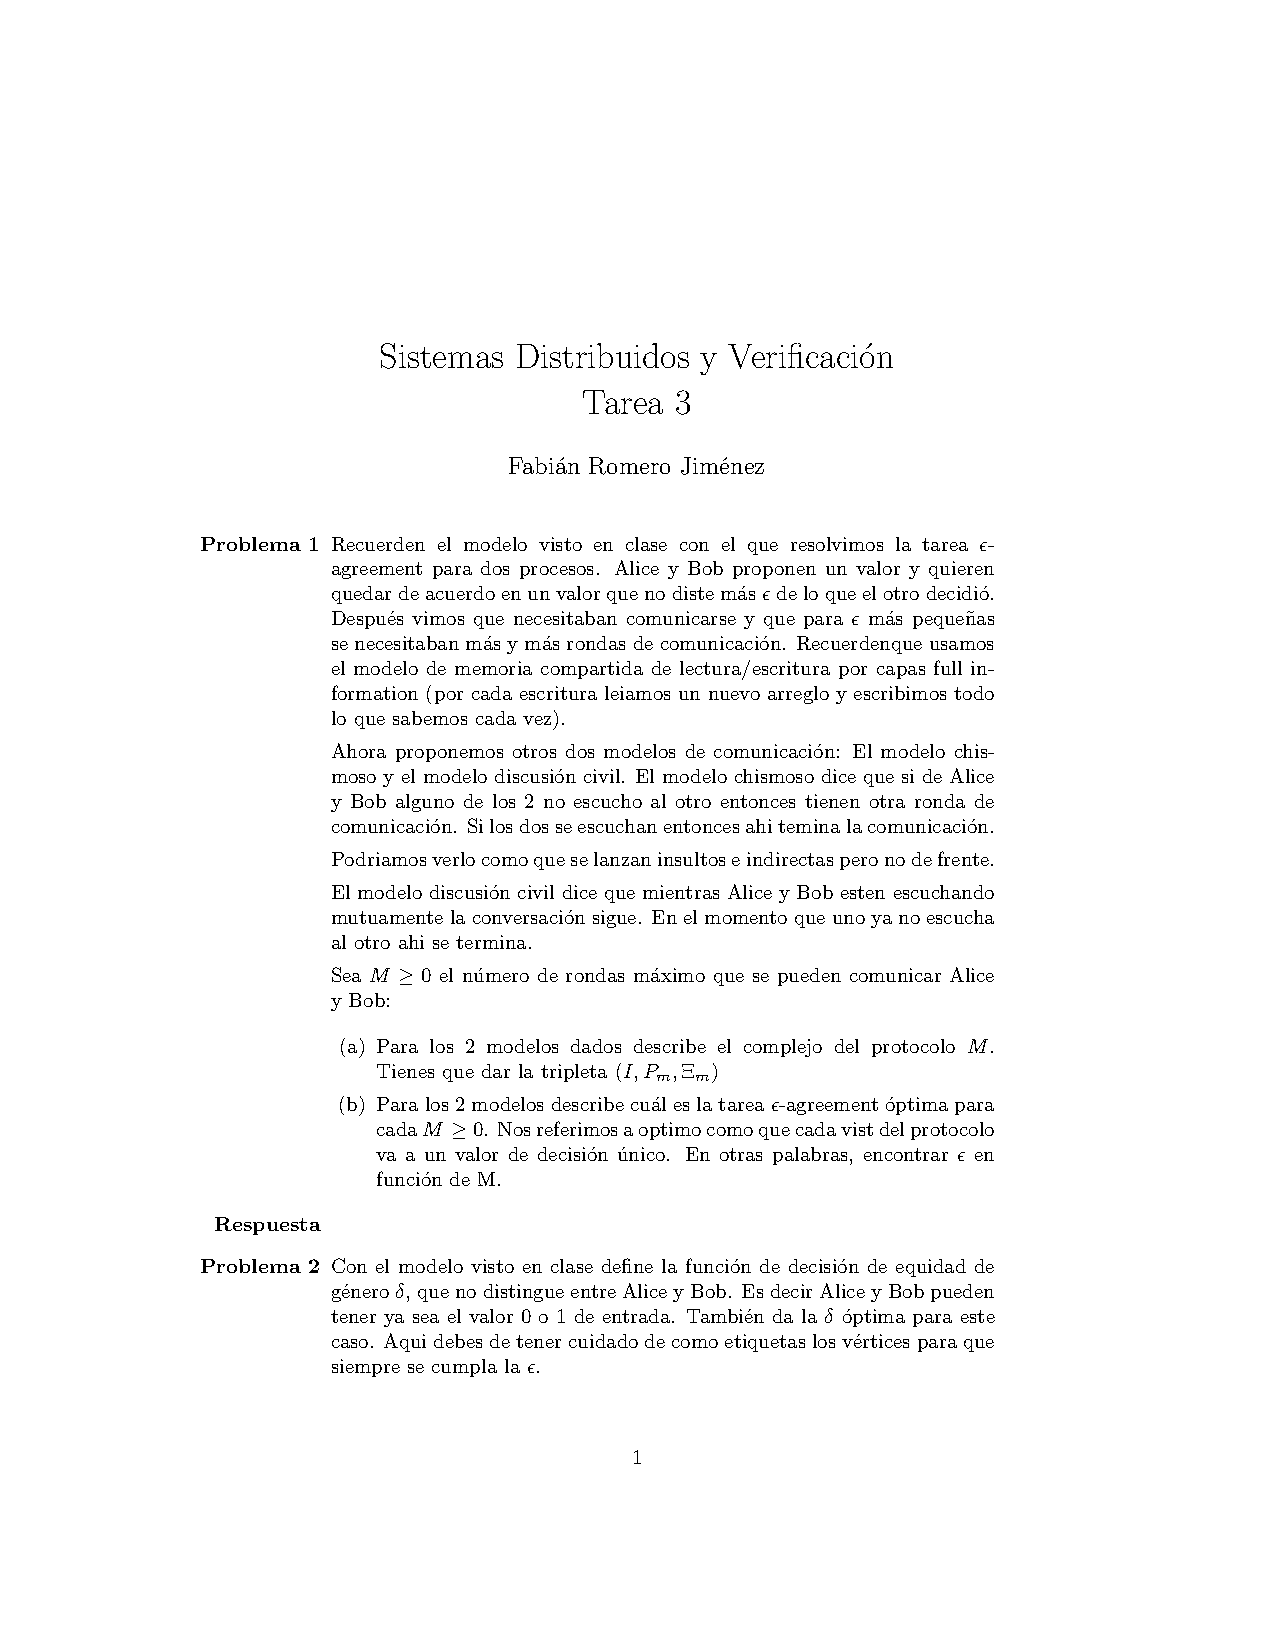
\includegraphics{t3.png}\\
  T3 con tres procesos dormidos que impide poner un cuarto proceso según el procedimiento.
\end{center}

\item Indique el número de vértices necesarios para un sistema de 8 hilos
e indique el número máximo de bits necesarios para representarlo.

Se puede representar cada nodo con un bit, y $T^k$ requiere $3$ veces los nodos que usa $T^{k-1}$ y como $|E(T^1)|=1=3^{0}$ se deduce por la relación de recurrencia que  $|E(T^k)|=3^{k-1}$ así $|E(T^8)|=3^{7}=2187$ que son tanto los nodos, como los bits necesarios para representar la gráfica.

\end{itemize}


\item[\bf{Problema 3}]Lee el documento de {\it Moore’s Law and the Sand-Heap Paradox} y da tu opinión en una cuartilla.

\item[\bf{Opinión}]

El artículo de Moshe Y. Vardi, plantea el problema de la ``muerte'' de la ley de Moore, en donde agrega que no solo es la densidad de transistores lo que cuenta, puesto que ``ya no es el caso que incrementando la densidad de transistores se aumenta también de forma automática el desempeño de las computadoras'' que es en mi opinion, un punto mucho mas importante, puesto que en realidad, el progreso en el desempeño es la fuerza de tracción detrás del avance tecnológico, el aumento de la densidad de transistores irrelevante por si mismo (especialmente si no trae consigo aumento en el desempeño).

Podemos hacer eco de la observación de Philip Wadler, que nos dice ``la concurrencia y la distribución son los problemas actuales más importantes de la computación. A medida que nos acercamos al 50 aniversario de la Ley de Moore, las reglas están cambiando: los recuentos de transistores en los núcleos de procesadores se duplican mientras que las velocidades de los relojes internos se mantienen fijas, lo que hace esencial la explotación de la concurrencia.'' y remata ``Sin una manera de construir de manera rutinaria y confiablemente sistemas distribuidos, medio siglo de progreso técnico sin precedentes, llegará a su fin.''

Tambien hay que notar que sin ese método ``rutinario y confiable'' de hacer programas que exploten eficientemente la concurrencia, no solamente se detendrá el progreso de los programas resultantes, sino que habrá cada vez menos incentivos económicos para que las empresas mejoren los procesos y arquitecturas de los procesadores, poniendo un alto tambien a todos los otros beneficios ``colaterales'' a la ley de Moore, como son memorias CMOS cada vez más grandes, discos duros con mayores capacidades, etc.

El artículo concluye con que nos acercamos a aguas inexploradas y que muchas cosas que damos por sentado en el progreso de la tecnología de computo. Por lo que el panorama se vuelve cuando menos turbio y desolador, a menos que encontremos eliminar la tiranía del ciclo de reloj como único motor de el aumento del desempeño.

\end{enumerate}

\end{document}
